\documentclass[10pt,a4paper,twoside,twocolumn]{article}
%% Lots of packages !
\usepackage{etex}

%% Francisation
\usepackage[english]{babel}
\usepackage[T1]{fontenc}
\usepackage[utf8]{inputenc}
%\usepackage{textcomp}

%% Réglages généraux
\usepackage[left=1.5cm,right=1.5cm,top=2cm,bottom=2cm]{geometry}
\usepackage{fancyhdr}
\usepackage{setspace}
\usepackage{lscape}
%\usepackage{multicol}
\usepackage{makeidx}
\usepackage[clearempty]{titlesec}
\usepackage{cite}

%% Packages pour le texte
\usepackage{pifont}
\usepackage{eurosym}
\usepackage{soul}
\usepackage[normalem]{ulem}
\usepackage{fancybox}
\usepackage{boxedminipage}
\usepackage{enumerate}
\usepackage{verbatim}
\usepackage{moreverb}
\usepackage{listings}
\usepackage[table]{xcolor}

%% Packages pour les tableaux
\usepackage{array}
\usepackage{multirow}
\usepackage{tabularx}
\usepackage{longtable}

%% Packages pour les dessins
\usepackage{graphicx}
\usepackage{wrapfig}
%\usepackage{picins}
\usepackage{picinpar}
\usepackage{epic}
\usepackage{eepic}
\usepackage{tikz}
\usepackage{afterpage}
\usepackage{rotating}
\usepackage{float}
\usepackage{caption}

%% Packages pour les maths
\usepackage{amsmath}
\usepackage{amssymb}
\usepackage{dsfont}
\usepackage{mathrsfs}
\usepackage{bussproofs}
\usepackage[thmmarks,amsmath]{ntheorem}

%% Création de nouvelles commandes
%\usepackage{calc}
\usepackage{ifthen}
\usepackage{xspace}



\usepackage{url}
\usepackage{hyperref}
\usepackage{todonotes}
\usepackage{subcaption}
\usepackage[french,ruled,vlined,linesnumbered,algosection,dotocloa]{algorithm2e}
\usepackage{MnSymbol}

\usepackage{chngcntr}

\usepackage{standalone}
\usepackage{import}

\usepackage[affil-it]{authblk}


\usepackage{lipsum}












\numberwithin{equation}{subsection}


\newcommand*{\rootPath}{../}
\standalonetrue

\begin{document}

\section{Density estimation methods}

Several methods exist to perform density estimation. Those methodes give result
with different level of quality for different computational cost. This section
will focus on describing some of those methods, which represent different
compromise.

\subsection{Methods description}

\subsubsection{CIC}

CIC\cite{Birdsall_Fuss_1969} (Cloud in cell) is the simpler and cheapest of all
methods presented in this paper. 

This method simply distribute each sample weight among the closest grid points.
This method has a very low computational cost ($\mathcal O(n)$) but suffer from
a very low quality in parse areas where each sample should be distributed over a
larger area, resulting in a lot of noise.

\subsubsection{AKDE}

AKDE\cite{Rosenblatt}\cite{Parzen1962} (Adaptive Kernel Density Estimator)
methods are the natural variant of CIC.

To try and solve the high quantity of noise, Kernel Density Estimator uses large
windows over which they distribute the weight of each sample. Those weight
follow a kernel function, typically gaussian function.

In order to avoid noise in parse areas and oversmoothing in dense areas, the
windows sizes are follow the local density. Windows adaptation criterions have
been extensivelly studied\cite{Heidenreich2013} but can, in some cases,
dramatically increass the computational cost.

Our implementation uses a kd-tree construction for selecting the window sizes.
Overall the complexity is $\mathcal O(n\log n + g^3)$ with far better results
then CIC (cf~\ref{ssect:method-results}).

\subsubsection{SPH}

\todo{to write}... %%%%%%%%%%%%%%%%%%%%%%%%%%%%%%%%%%%%%%%%%%%%%%%%% TODO

\subsubsection{Tess-Dense}

Unlike all previous algorithm, Tess-Dense doesn't use fixed shape windows.
Indeed, Tess-Dense uses a voronoï tesselation to determine each sample influence
domaine\todo{ref - Self-Adaptive Density Estimation of Particle Data}. This
precomputation is independant of the result grid's resolution therefore reducing
the memory footprint on high resolution reconstruction. This cost is however
paid even for small resolutions.

The cost of this method is $\mathcal O(n^2 + g^3)$. While produced results are
good, they suffer from some noise caused by voronoï cells' instability in sparse
areas.

\subsection{Methods results} \label{ssect:method-results}

To compare thoses different methods results we plot the frequencial reponse of
their result and compare them to the analytical result. One should not forget
that the input set of those methods are sampling of a density function. As those
sampling are inherently random, we cannot just observe on sampling and the
associated result.

In order to take this randomness into account we computed several samplings of
our density function model and then display both the median of the frequencial
results overs thoses samplings as well as extreme values. That way we can not
only describe the expected quality of those methods but also the natural
variability we can expect. Figure~\ref{fig:synthetic:spectral} present thoses
results for all prevously described methods processing synthetic samplings
produced by our analitical model.

\begin{figure}[!ht]
	\centering
	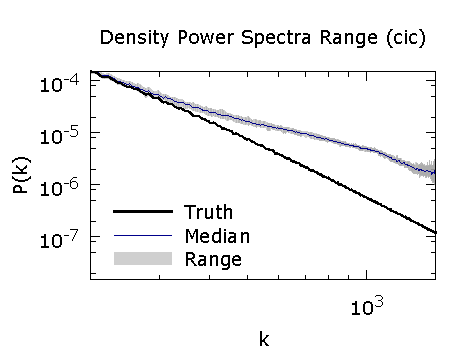
\includegraphics[width=0.24\textwidth]
		{\rootPath Figures/synthetic/psd-methods/cnfw_particles_2e5_cic_clamped.pdf}
	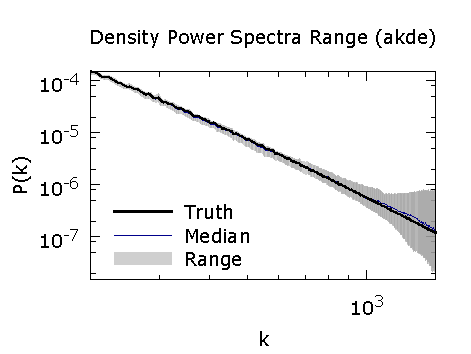
\includegraphics[width=0.24\textwidth]
		{\rootPath Figures/synthetic/psd-methods/cnfw_particles_2e5_akde_clamped.pdf}
	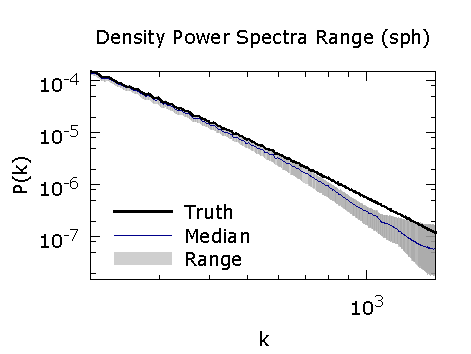
\includegraphics[width=0.24\textwidth]
		{\rootPath Figures/synthetic/psd-methods/cnfw_particles_2e5_sph_clamped.pdf}
	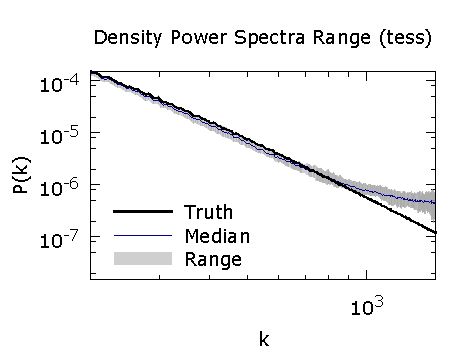
\includegraphics[width=0.24\textwidth]
		{\rootPath Figures/synthetic/psd-methods/cnfw_particles_2e5_tesscic_clamped.pdf}
	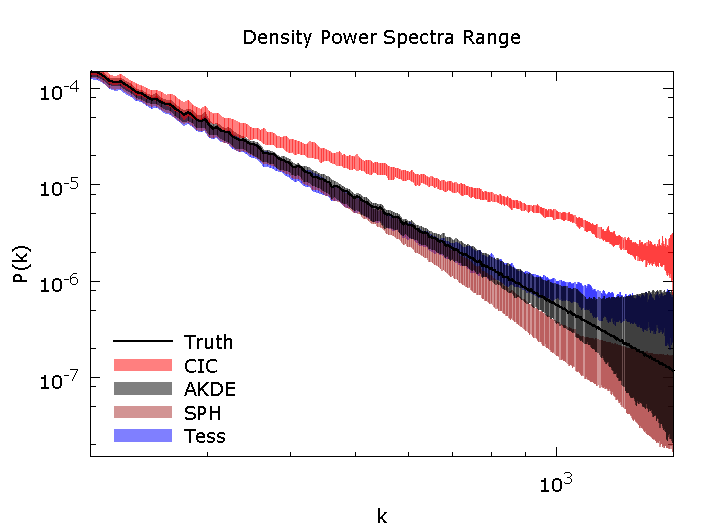
\includegraphics[width=0.48\textwidth]
		{\rootPath Figures/synthetic/psd-methods/cnfw_particles_2e5_full.pdf}
	\caption{Spectral analysis of density estimation methods processing synthetic
		samplings from or analytical model}
	\label{fig:synthetic:spectral}
\end{figure}

Thoses results clearly shows the noisiness of CIC. As for the other methods,
they give different shape of results with different level of variability while
not showing one as clearly better than the others.

Tess-Dense's slight noisiness might be related to the use of flat weight
distribution among each cell's inner grid point. Secondary methods used for
weight distribution in dense area are also subject to some aliasing and
therefore noise.

On the AKDE/SPH side, we mostly notice a high intrinsic variability. That may be
caused by the sampling's random variation affecting the window size computation
in such a way that we could locally encounter noisyness or oversmoothness.

\begin{table*}[!ht]
	\centering
	\begin{tabular}{|l|c|c|c|c|c|}
		\hline
								& Analytical	& CIC				& AKDE			& SPH				& Tess-Dense\\
		\hline
		Analytical	& --					& $0.00314$	& $0.00049$	& $0.00214$	& $0.00194$	\\
		CIC					&	$0.00314$		& --				& $0.00338$	& $0.00513$	& $0.00435$	\\
		AKDE				&	$0.00049$		&	$0.00338$	& --				& $0.00179$	& $0.00151$	\\
		SPH					&	$0.00214$		&	$0.00513$	& $0.00179$	& --				& $0.00099$	\\
		Tess-Dense	&	$0.00194$		&	$0.00435$	& $0.00151$	& $0.00099$	& --				\\
		\hline
	\end{tabular}
	\caption{Distance between density estimation methods processing synthetic
		samplings from or analytical model}
	\label{table:syntetic:distance}
\end{table*}


Running those methods on Hacc's results show similar results as figure~
\ref{fig:hacc:spectral} shows. Note that, as Hacc is producing a single sample
for each time step, we don't have multiple samples to compare as we do with our
synthetic particles generator. That is why figure~\ref{fig:hacc:spectral} does
not show variability range for thoses results.

\begin{figure}[!ht]
	\centering
	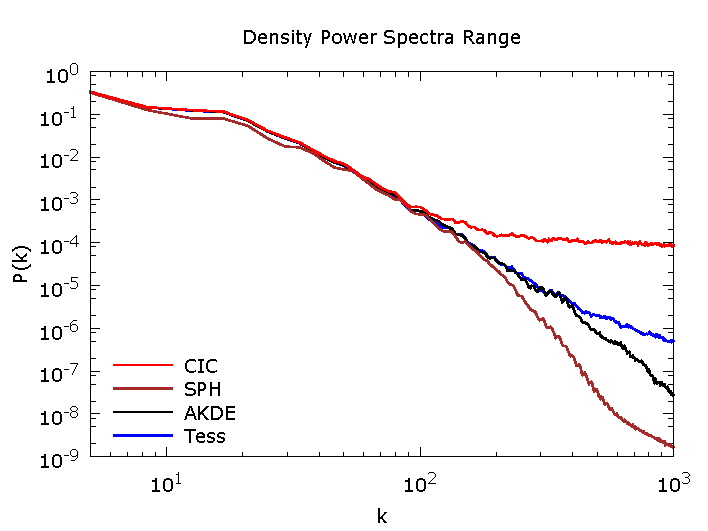
\includegraphics[width=0.48\textwidth]
		{\rootPath Figures/hacc/psd-methods/trace_255_full.pdf}
	\caption{Spectral analysis of density estimation methods processing an
		experimental samplig produced by Hacc}
	\label{fig:hacc:spectral}
\end{figure}

\begin{table*}[!ht]
	\centering
	\begin{tabular}{|l|c|c|c|c|c|}
		\hline
								& CIC				& AKDE			& SPH				& Tess-Dense\\
		\hline
		CIC					& --				& $0.02313$	& $0.07020$	& $0.02190$	\\
		AKDE				&	$0.02313$	& --				& $0.04709$	& $0.00563$	\\
		SPH					&	$0.07020$	& $0.04709$	& --				& $0.04851$	\\
		Tess-Dense	&	$0.02190$	& $0.00563$	& $0.04851$	& --				\\
		\hline
	\end{tabular}
	\caption{Distance between density estimation methods processing an
		experimental samplig produced by Hacc}
	\label{table:hacc:distance}
\end{table*}


%=====================================================================
%=====================================================================
\ifstandalone
	\bibliographystyle{apalike}
	\bibliography{\rootPath Annexes/biblio}
\fi
%=====================================================================
%=====================================================================
\end{document}
